\documentclass[12pt]{report}
\usepackage[utf8]{inputenc}
\usepackage[OT1]{fontenc}
\usepackage{lmodern}
\usepackage[a4paper, total={6in, 8in}]{geometry}
\usepackage{setspace}
\usepackage{parskip}
\usepackage{fancyhdr}

\usepackage{graphicx}
\usepackage{tikz}
\usepackage{dirtree}
\usepackage{graphviz}
\usepackage{multicol}
\usepackage{mdframed}



\usepackage{listings}
\usepackage{minted}
\usepackage{booktabs}
\usepackage{makecell}
\usepackage{tabularx}
\usepackage{caption}
\usepackage{todonotes}

\usepackage{biblatex}
\addbibresource{references.bib}

\usepackage[hidelinks]{hyperref}
\usepackage[toc]{glossaries}

\graphicspath{{../images/}}

% Page style
\emergencystretch=1em

\setlength{\headheight}{44.0pt}
\fancyhead{}
\fancyhead[L]{\rightmark}
\fancyfoot{}
\fancyfoot[R]{\thepage}

\newcommand{\confer}[1]{~(cf.~page~\pageref{#1})}


\onehalfspacing{}
\setlength{\marginparwidth}{2cm} 
\usetikzlibrary{positioning,shapes,arrows}

\definecolor{bg}{rgb}{0.95,0.95,0.95}

\setminted{autogobble, breaklines, frame=lines, framesep=2\fboxsep, tabsize=2, framerule=0.2pt, fontsize=\footnotesize}

\newglossaryentry{security}{
    name=security,
    description={A security is a financial asset that can be bought and sold. Stocks, options and debt notes are all securities. Every security has an Issuer. A loan from a bank is not a security, because the bank can not generally sell the loan to another bank.},
    plural=securities
}

\newglossaryentry{asset}{
    name=asset,
    description={An asset is something that can eventually generate cashflows. Because not all future cashflows are known with certainty, the value of an asset must be discounted to reflect the risk that those cashflows do not meet expectations.},
    plural=assets
}

\newglossaryentry{issuer}{
    name=issuer,
    description={Companies are issuers of securities.},
    plural=issuers
}

\newglossaryentry{stock}{
    name=stock,
    description={Stocks are securities that represent ownership in a company. Stock are typically issued as shares (e.g. 100 shares of Apple stock). Shares are fractions of a company's total ownership.}
    plural=stocks
}

\newglossaryentry{debt}{
    name=debt,
    description={Debt is a loan that must be repaid. Companies might raise funds via equity issuances or debt issuances. Debt is issued as security in terms of the amount that was loaned, the interest rate, and the maturity date. Debt is safer than equity, and must be repaid before equity holders can receive any cashflows.},
    plural=debt
}

\newglossaryentry{convertible-debt}{
    name={convertible debt},
    description={In startup financing, it is typical to encounter convertible debt. Convertible debt is a loan that can be converted into equity at a later date. The conversion is typically triggered by a future financing round. The conversion price is typically set at a discount to the price of the future financing round. Since debt is safer, convertible debt has lower investment risk. Conversion is typically at the option of the holder.},
    plural={convertible debt}
}

\newglossaryentry{stock-option}{
    name={stock option},
    description={Stock options are securities that give the right for their holder to purchase stock at a predefined price (the strike price) at a predefined date (the maturity date). The value of a stock option is the different between the market price for the stock and the strike price. Stock options are typically issued to employees as part of their compensation package.},
    plural={stock options}

}

\newglossaryentry{startup-company}{
    name={startup company},
    description={A startup company is a new company that is searching for a business model as it grows. Startup companies are typically funded in stages and by specialized venture capital investors such as individual (angel) investors and funds. Startup companies usually aim for high growth and high returns, by choosing projects with higher risk.},
    plural={startup companies}
}

\newglossaryentry{capitalization-table}{
    name={capitalization table},
    description={A capitalization table is a table that lists all the securities issued by a company. The capitalization table lists the number of shares issued, the type of security, the price per share, and the date of issuance. The capitalization table is used to calculate the ownership of each shareholder.},
    plural={capitalization tables}
}

\newglossaryentry{vesting-period}{
    name={vesting period},
    description={A vesting period is a period of time during which an employee must remain employed in order to receive the full value of their stock options. Vesting periods are typically 4 years, with a 1 year cliff period. Only vested stock options can be execised.},
    plural={vesting periods}
}


\newglossaryentry{cliff-period}{
    name={cliff period},
    description={The cliff period is the period of time before which no stock options are vested. After the cliff period, stock options are typically vested monthly.},
    plural={cliff periods}
}

\newglossaryentry{strike-price}{
    name={strike price},
    description={The strike price is the price at which a stock option can be exercised. The strike price is typically set at the market price of the stock at the time of issuance, but may be futher discounted to incentivize employees.},
    plural={strike prices}
}

\newglossaryentry{common-stock}{
    name={common stock},
    description={Stock that holds no special rights beyond a share in profits. Common stock is the most common type of stock.},
    plural={common stock}
}

\newglossaryentry{preferred-stock}{
    name={preferred stock},
    description={Preferred stock is stock that holds special rights. As an example of a special right, preferred stock might have a guaranteed dividend payment but less voting rights.},
    plural={preferred stock}
}

\newglossaryentry{stakeholder}{
    name={stakeholder},
    description={A stakeholder is any person, legal or natural, with an economic interest in a company, including all debt, option and stock holders.},
    plural={stakeholders}
}

\newglossaryentry{share}{
    name={share},
    description={Shares represent a fraction of ownershp in a company. The number of shares a stock holder owns is the starting point for calculating their ownership stake in the company.},
    plural={shares}
}

\newglossaryentry{exercise}{
    name={exercise},
    description={Stock options are exercised and become stocks. The strike price is the price at which the stock options can be converted to equity. They can only be exercised after they have been vested.},
    plural={exercises}
}

\newglossaryentry{staged-financing}{
    name={staged financing},
    description={Staged financing is a financing strategy in which a company raises funds in stages. The first stage is typically called the seed round, with subsequent stages receiving a latin alphabet letter (such as Series A, Series B, etc.). Staged financing allows investors to reduce their risk by investing in stages, and allows the company to raise funds as it grows.},
    plural={staged financing}
}

\newglossaryentry{financing-round}{
    name={financing round},
    description={Each stage of financing is also called a financing round. Each financing round is typically led by a lead investor, who sets the terms of the financing round. The terms of the financing round include the valuation of the company, the price per share, and the type of security issued.},
    plural={financing rounds}
}
\newglossaryentry{sweat-equity}{
    name={sweat equity},
    description={Startup founders raise capital by selling shares of their stock to investors. For example, a investor might take 20 of 100 shares, leaving founder with 80 shares that were not issued against cash. This complement of the shares that held by investors is called sweat equity.},
    plural={sweat equity}
}

\newglossaryentry{dilution}{
    name={dilution},
    description={Dilution is the reduction in ownership stake that occurs when new shares are issued. In the special case that in the financing round investors purchase new shares proportionally to their then current stake, no dilution occurs. Founders and employees can also be diluted by the issuance of new shares.},
    plural={dilution}
}

\newglossaryentry{asset-class}{
    name={asset class},
    description={An asset class is a group of securities that have similar characteristics. Stocks, bonds, and real estate are all asset classes.},
    plural={asset classes}
}

\newglossaryentry{stock-class}{
    name={stock class},
    description={A stock class is a group of stocks that have similar characteristics. Common stock and preferred stock are both stock classes.},
    plural={stock classes}
}

\newglossaryentry{transaction}{
    name={transaction},
    description={A transaction refers to the issuance, change, transfer and cancellation of securities. A transaction is typically initiated by a stakeholder, and must be approved by the company. Most transactions involve a cost, with money changing hands in the opposite direction of the securities.},
    plural={transactions}
}

\newglossaryentry{equity}{
  name={equity},
  description={Equity represents ownership interest in a company. It can come in the form of stocks or stock options and may be granted to founders, employees, or investors. Equity holders have a claim to the profits of the company.},
  plural={equity}
}

\newglossaryentry{venture-capital}{
  name={venture capital},
  description={Venture capital is a form of private equity financing that is provided by venture capital firms to startups and early-stage companies that have been deemed to have high growth potential or which have demonstrated high growth},
  plural={venture capital}
}

\newglossaryentry{angel-investor}{
  name={angel investor},
  description={An angel investor is an individual who provides capital for a business start-up, usually in exchange for convertible debt or ownership equity. These investors typically support startups in the early stages of growth},
  plural={angel investors}
}

\newglossaryentry{liquidity-event}{
  name={liquidity event},
  description={A liquidity event is an event that allows a company's stakeholders to cash out or make a profit from their investment. This could be a sale of the company (also known as an exit), an IPO, or a large dividend distribution},
  plural={liquidity events}
}

\newglossaryentry{issuance}{
  name={issuance},
  description={An issuance is the creation of a new security}
  plural={issuances}
}

% An entry for IPOs
\newglossaryentry{ipo}{
  name={initial public offering},
  description={During an initial public offering, a company sells shares of its stock to the public for the first time. This is also known as "going public" and is a way for companies to raise capital for new investments or to pay off existing debt.},
  plural={initial public offerings}
}

% acquisition
\newglossaryentry{acquisition}{
  name={acquisition},
  description={An acquisition is when one company purchases another company. Depending on how many shares are acquired, the acquiring company may gain control of the acquired company.},
  plural={acquisitions}
}

\renewcommand*{\glstextformat}[1]{{\textbf{#1}}}

\makeglossaries{}

\begin{document}

\begin{titlepage}
\begin{center}

\makebox[\textwidth][c]{
\includegraphics[width=0.5\textwidth]{images/ime_usp_logo.png}}

\vspace{1cm}

\textbf{Universidade de São Paulo} \\
\textbf{Institute of Mathematics and Statistics} \\
\textbf{Department of Computer Science}

\vspace{1.5cm}
\textbf{\LARGE A Formalization of a Startup Finance Transaction Model using Alloy}

\vspace{1.5cm}

\textbf{\Large Rodrigo Ehrlich Stevaux}

\vspace{1cm}

\textbf{\Large Advisor: Prof.\ Ana Cristina Vieira de Melo}

\vspace{1cm}
\begin{flushright}
    \begin{minipage}{0.5\textwidth}
        \begin{flushleft}
            Dissertation presented to the Institute of Mathematics and Statistics at the University of São Paulo, as part of the requirements for the degree of Master of Science in Computer Science
        \end{flushleft}
    \end{minipage}
\end{flushright}

\vspace*{\fill}

\textbf{\large São Paulo}

\vspace{0.5cm}
\textbf{\large 2023}

\end{center}
\end{titlepage}

\newpage
\thispagestyle{empty}
\
\newpage
This paper proposes a formal model for a subset of the startup finance transaction space. The initial version of the provided domain is the result of an industry coalition effort to make the data model standard.

The data definition explains how this domain can be modeled syntactically. We refined this first model with semantics on transactions by using the Alloy formal modeling language and analyzer, aiming for a more expressive and correct model by capturing domain invariants. As a result, the new model is machine-checkable for important safety integrity criteria.

This research contributes to the field of formal methods by demonstrating how to progress from a semi-formal specification to a formal one, evaluating the results, and providing a case study of a real-world domain.
\newpage

I dedicate this thesis to my late, loved mother, and to my father.

\vspace{1em}

I thank my advisor, Prof.\ Ana Cristina Vieira de Melo, not only for her academic guidance and support throughout this work, but for the friendship and care she has shown me since during this endeavor.

I am grateful to my institution for providing me with the opportunity to pursue this work, and from all I have learned from my colleagues and professors.

I thank all the people who helped me arrive at this point, including my family, friends, and colleagues.

\tableofcontents

\listoffigures
\listoftables
\listoflistings{}

\glsaddall{}
\printglossary{}

\part{Background}

\include{ch-intro}
\include{ch-cap-tables}

\part{Models}



\chapter{Towards an improved specification for capitalization tables based on the Open Cap Table format}\label{ch:towards}

\section{Requirements of a consistent model for capitalization tables}

A consistent model for \glspl{capitalization-table} should be able to guarantee that the following requirements hold:

\begin{itemize}
	\item The total number of shares in circulation must never exceed the number of shares issued by the issuer.
	\item \Glspl{issuance} create new shares, transfers do not create new shares, cancellations destroy shares.
	      \begin{itemize}
		      \item Cancellations and transfers fully consume their input security. A balance \gls{security} is created in case of partial cancellations or transfers
		      \item Securities must either be issued or be a result or balance \gls{security} of a transfer or the balance \gls{security} of a cancellation
	      \end{itemize}
	\item Every \gls{security} is owned by one and only one \gls{stakeholder}
	\item Every \gls{security} can be traced back to a single \gls{issuance}.
	\item Every \gls{security} in a \gls{stakeholder}'s portfolio can be traced back to the transaction that issued it to the \gls{stakeholder} or that transferred it to the \gls{stakeholder}
\end{itemize}

There is nothing exceptional about these requirements.

They are naturally expected in the accounting and finance domain. However, they are not enforced by the Open Cap Table format, and could not be, given the limitations of JSON Schema.

\section{Expressiveness of the contracts and vesting rules}

The greatest complexity in validating the transactions that compose a \gls{capitalization-table} lies in employee stock option plans. Stock options awarded to employees are subject to vesting rules, which are usually complex and vary from company to company.

The variety of vesting rules that can be found in actual stock option grants are written in legal documents, and limited only by the creativity of lawyers.

Therefore, a model for \glspl{capitalization-table} should be able to express a range of vesting rules. The vesting rules that can be expressed by the Open Cap Table format can be improved simply by adding a propositional logic layer to the vesting rules.

\section{An introduction to Alloy}

Alloy, first introduced by Daniel Jackson in 2002~\cite{jackson-2002}, is today a complete framework for modeling and analyzing software systems. We say it is a framework because it is composed of more than just a modeling language.

The idea underlying Alloy is that ``software should be built on abstractions'', and that by picking the right ones, programming should ``naturally from design''.

Alloy is distributed as the Alloy Analyzer, which features:

\begin{itemize}
	\item A modeling language
	\item A visualizer for metamodels and model instances
	\item A bounded model checker
	\item A standard library for common data structures (sequences, graphs, relations, etc.)
\end{itemize}

By combining the three features above, an Alloy user can quickly iterate on a model, visualize and explore instances, and express and check properties. An Alloy model can focus both on the concepts underneath the system being modeled, on the data model and relationships, and on more operational aspects of the system by modeling relations between two or more states.

\subsection{Parts of an Alloy model}

Every alloy model is composed of signatures, predicates, facts, functions, assertions, and commands:

\begin{enumerate}
	\item Signatures: the basic building blocks of Alloy models, they represent entities in the domain. Signatures have \textit{fields} that relate them to other signatures.
	\item Functions: A function in Alloy relates instances of signatures to relations. An alloy function is a function like in any programming language.
	\item Predicates: A predicate in Alloy is a function that returns a boolean value. Predicates are used to express properties of the model.
	\item Facts: A fact is a predicate that must always be true in the model. A fact actively constrains the model by discarding instances that do not satisfy it.
	\item Assertions: An assertion is a predicate that can be given to a check command, and expresses our \textit{expectations} of the model. Assertions do not constrain the model effectively.
	\item Commands (Checks and runs): The \verb|run| finds \textit{examples} of the model that satisfy all constraints, while the \verb|check| command finds \textit{counter-examples} that violate a given assertion.
\end{enumerate}

To illustrate the concepts above, we give a very model and analyze its parts.

\begin{listing}[H]
\begin{minted}{alloy}
sig Stakeholder {
    portfolio : set Security
}

sig Security {
    owner : one Stakeholder
}

fact invOwnerPort { ~owner = portfolio }

pred overlap[s1, s2 : Stakeholder] {
    s1.portfolio & s2.portfolio != none
}

assert noSharedOwnership {
    no disj s1, s2 : Stakeholder | overlap[s1, s2]
}
\end{minted}
\caption{A simple Alloy model}
\label{lst:alloy-model}
\end{listing}

In our case, there are signatures for two concepts in our domain: \glspl{security} and stakeholders, which own \glspl{security} by having a portfolio.

We can note that Alloy gives more control over the cardinality of relationships than a class or table: \verb|portfolio| is a set of \verb|Security|, and not a single \verb|Security|.

The fact states that \verb|owner| and \verb|portfolio| are inverses of each other (their union forms a symmetrical relation), which is a constraint that must always hold in the model. Alloy uses the \verb|~| operator to denote the inverse of a relation.

The predicate \verb|overlap| tells us whether two different \glspl{stakeholder} can any \gls{security} in common in the portfolio, which we would not expect in a real-world scenario.

The \verb|noSharedOwnership| assertion tells us that there are no two \glspl{stakeholder} that own the same security.

\subsection{Using the Alloy Analyzer}

The user can analyze an Alloy model by checking whether certain assertions hold, or by running simulations of instances of the model. Alloy can find counterexamples to assertions, and can also find instances that satisfy certain properties.

We can ask Alloy to check whether the assertion \verb|noSharedOwnership| holds by issuing a check command (for a scope of size 5):

\begin{listing}
	\begin{minted}{alloy}
		check noSharedOwnership for 5
	\end{minted}
	\caption{Checking an assertion}
	\label{lst:alloy-check}
\end{listing}

We explicitly ask Alloy to use a scope of 5, meaning there will be at most 5 stakeholders, 5 \glspl{security}.  It is essential to bounded-model checking to give a bound.

After a few tenths of a second, Alloy will tell us that the assertion holds, by stating that it couldn't find a counterexample:

\begin{listing}\label{lst:alloy-check-output}
	\begin{verbatim}
Executing "Check noSharedOwnership for 5"
Solver=minisatprover(jni) 
    Bitwidth=4 MaxSeq=5 
    SkolemDepth=4 Symmetry=20 Mode=batch
Generating CNF...
820 vars. 70 primary vars. 1280 clauses. 193ms.
Solving...
No counterexample found. Assertion may be valid. 16ms.
core reduced from 8 to 6 top-level formulas. 138ms.
\end{verbatim}
	\caption{Alloy's output}
\end{listing}

\newpage

Finally, we can issue a \verb|run| command to find instances of the model that satisfy the constraints:

\begin{listing}[H]\label{lst:alloy-run}
	\begin{minted}{alloy}
run {} for 5 but exactly 2 Stakeholder, 5 Security
\end{minted}
	\caption{Running the model}
\end{listing}

A sample visualization generated by the run command is show below in figure~\ref{fig:alloy-run}.

\begin{figure}[H]
	\centering
	\fbox{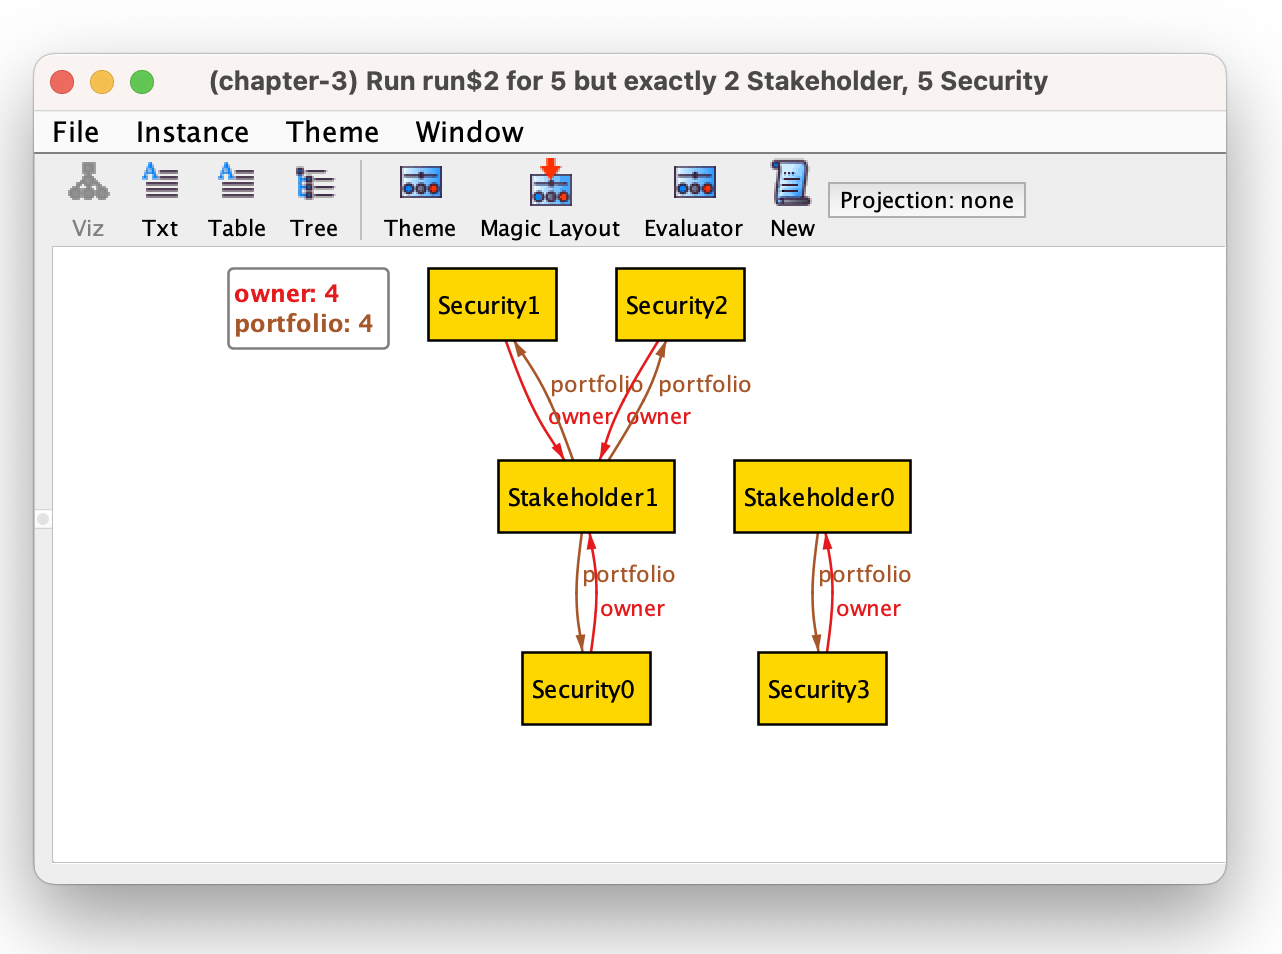
\includegraphics[width=0.8\textwidth]{images/alloy-run.png}}
	\caption{A sample instance generated by Alloy}\label{fig:alloy-run}
\end{figure}

\subsection{Refining a model}

We know the model is correct (up to a bound). But why? We can use Alloy to find out.

\newpage

The technique is to turn the \verb|invOwnerPort| fact into a \textit{predicate}; meaning that we do not assume it holds. But we can still ask Alloy to check whether it \textit{suffices} for \verb|noSharedOwnership| to hold, with a small change in the model:

\begin{listing}[H]\label{lst:alloy-strengthen}
	\begin{minted}{alloy}
pred invOwnerPort { ~owner = portfolio }
\end{minted}
	\caption{Strengthening the model}
\end{listing}

Now, the \verb|noSharedOwnership| assertion does not hold anymore, since we can find a counterexample:

\begin{listing}[H]\label{lst:alloy-strengthen-output}
	\begin{verbatim}
Executing "Check noSharedOwnership for 5"
Solver=minisatprover(jni) 
    Bitwidth=4 MaxSeq=5 
    SkolemDepth=4 Symmetry=20 Mode=batch
Generating CNF...
767 vars. 70 primary vars. 1177 clauses. 85ms.
Solving...
Counterexample found. Assertion is invalid. 14ms.
\end{verbatim}
	\caption{Alloy's output with a counterexample after strengthening the model}
\end{listing}

We call \verb|check| with a modified assertion, namely:

\begin{listing}[H]\label{lst:alloy-strengthen-check}
	\begin{minted}{alloy}
check noSharedOwnershipAlt {
    invOwnerPortfolio implies {
        no disj s1, s2 : Stakeholder | overlap
    }
}
\end{minted}
	\caption{Checking the model again, considering the strengthened assumptions}
\end{listing}

\newpage

Now we see that the model is still correct. That holds, but only because of the \verb|invOwnerPortfolio| predicate:

\begin{listing}[H]\label{lst:alloy-strengthen-check-output}
	\begin{verbatim}
Executing "Check noSharedOwnershipAlt"
Solver=minisatprover(jni) 
    Bitwidth=4 MaxSeq=4 
    SkolemDepth=4 Symmetry=20 Mode=batch
Generating CNF...
318 vars. 30 primary vars. 476 clauses. 104ms.
Solving...
No counterexample found. Assertion may be valid. 6ms.
core reduced from 8 to 6 top-level formulas. 23ms.
\end{verbatim}
	\caption{Alloy's output showing no counterexample after considering the strengthened assumptions}
\end{listing}

There is much going on underneath Alloy to make this possible, ultimately relying on the KodKod library~\cite{TorlakJackson2007} to translate Alloy problems to and from SAT problems.

A full presentation of Alloy is beyond the scope of this work, but can be found in the Software Abstractions book by Daniel Jackson~\cite{jackson-2012}.

\section{From JSON Schema to Alloy}

The OCF is chiefly a data format, while we are looking for a conceptual model. Nevertheless, the OCF is a good starting point for a conceptual model, and we can use it to derive a conceptual model that is more expressive and that can be used to validate capitalization tables.

The general approach has the following steps:

\begin{enumerate}
	\item Define the signatures roughly matching the documents in the JSON Schema, even if we must declare them as abstract before refining them
	\item Refine the signatures by adding fields and constraints, based on the keys and values in the JSON Schema
	\item Add expected properties (of the model) as assertions composed of predicates
	\item Check that assertions hold, or debug the model until they do
\end{enumerate}

Step 1 is very mechanical and straightforward. Step 2 requires some attention to detail, since relations in JSON schema are very different from those in Alloy. JSON Schema mostly defines JSON objects, which are associative maps. Some documents define an array of objects, or refer to other documents by ID.~On the other hand, Alloy provides fine-grained control over the arity and multiplicity of relations. Step 3 requires domain expertise and some training in the background relations, set and logic, and some creativity. Step 4 is a matter of running the Alloy Analyzer and checking the results, plus some debugging.

The whole process is not exceedingly difficult to perform, specially if compared to alternatives, Such as Z, TLA$^{+}$, or dependently typed languages and proof assistants such as Agda, Coq or Idris. It resembles writing SQL schemas or business domain entities in object-oriented languages, but it does require some familiarity with mathematics (set theory and logic).

\section{A brief overview of Alloy related literature}

Alloy is cited in more than 1,200 papers, with many extensions and applications
in software design and modeling. Alloy$\ast$ is a higher-order extension of
Alloy that can be used for program synthesis, since it supports higher-order
quantification~\cite{Milicevic2017}. $\alpha{Rb}y$ is an embedding of Alloy in
Ruby~\cite{Arby}.

A number of other modeling languages have been translated to or partially modeled in Alloy\cite{alloy-case-studies}, including UML, $i^\star$, CVL, Event-B and, Z, OCL.\@Alloy can also be used with verification languages such as ACL2 or Isabelle.

Alloy has been used in a wide range of applications in software engineering, database design, \gls{security} analysis~\cite{Carpio2021}\cite{Chen2006}, multiagent negotiations~\cite{Podorozhny}. It has also been applied to modeling beyond computer science, such as a model for central bank policy~\cite{Johnson2021}. A model of the same-origin-policy used in web browsers can be found in the 500 Lines or Less open-source book~\cite{500Lines19:online}.

\textit{We were unable to find previous models of \glspl{capitalization-table} in Alloy.}

\include{ch-transaction-tracing}
\chapter{A model for enhancing the expressiveness of vesting rules}\label{ch:vesting-system}

In this chapter, we will walk through the Alloy model, which enhances upon an open-source JSON Schema model. We incorporate and demonstrate the use of And/Or/Not operators, thus extending the triggers to more of a domain-specific language that supports propositional logic. In particular, we leverage the not operator with the ExactDate trigger to express the ``until condition'', which allows the model to express contract clauses that stipulate a milestone to be achieved until a given date.

The model is shown in Figure~\ref{fig:vs-metamodel}.
\begin{figure}[H]
	\centering
	\fbox{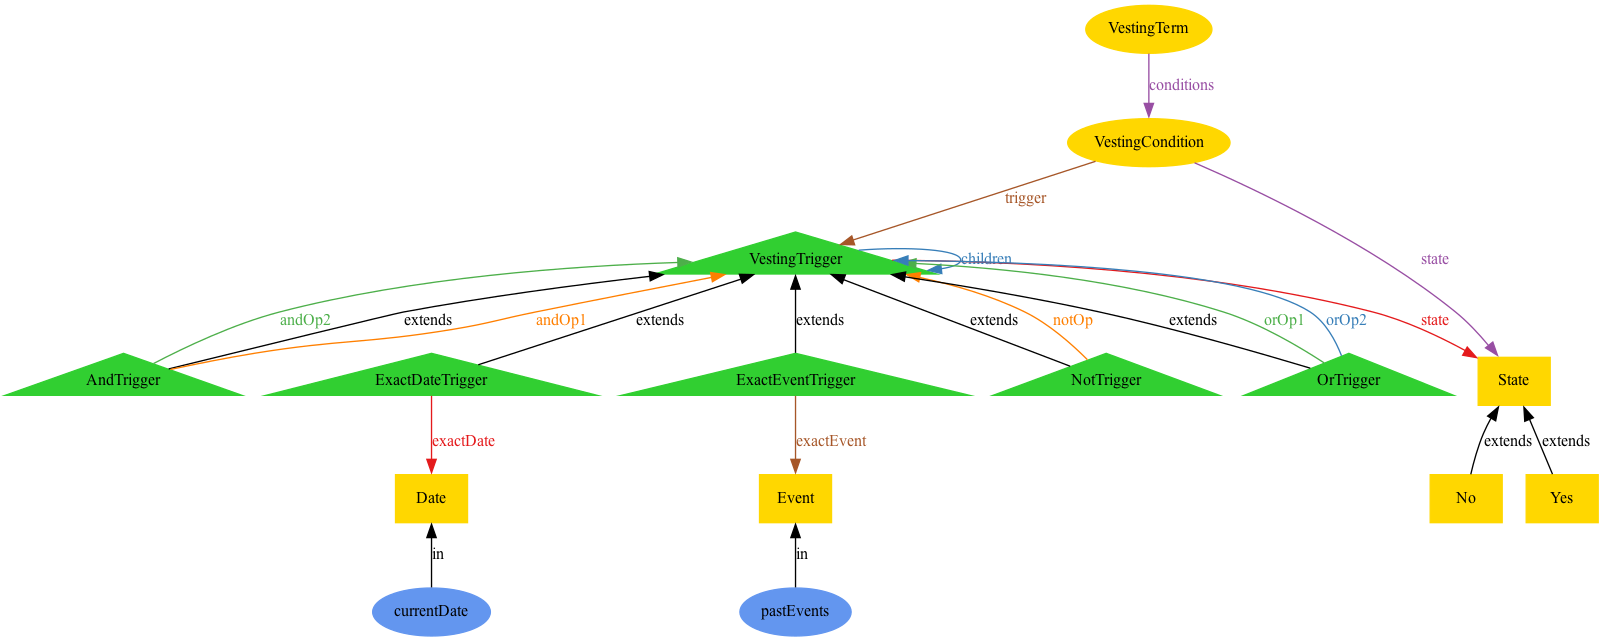
\includegraphics[width=\textwidth]{images/metamodel4.png}}
	\caption{Vesting system metamodel}\label{fig:vs-metamodel}
	As rendered by the Alloy Analyzer
\end{figure}

\section{Vesting Terms and Conditions}

Our Alloy model begins with the definition of the \verb|VestingTerm|, \verb|VestingCondition| and \verb|VestingTrigger| signatures.

A \verb|VestingTerm| represents a set of conditions that need to be met and the authorized shares for the vesting term. The \verb|VestingCondition| signifies a particular condition or a trigger.

Since our modeling has no form of mutation involved, there is no need to identify a vesting term with a vesting condition \textemdash{whether other vesting terms refer to the same conditions is harmless, as long as the authorized shares match the shares in the conditions}.

\begin{listing}[H]\label{listing:vs:vesting-term}
	\begin{minted}{alloy}
	sig VestingTerm {
		conditions : set VestingCondition,
		authorizedShares : Int
	}
	\end{minted}
	\caption{Vesting term signature}
\end{listing}

\begin{listing}[H]\label{fig:vs:vesting-condition}
	\begin{minted}{alloy}
sig VestingCondition {
    trigger : VestingTrigger,
    state : State,
    shares : Int
}
\end{minted}
	\caption{Vesting condition signature}
\end{listing}

This fact relating shares in vesting terms and shares in vesting conditions is not expressible in JSON Schema because it is a constraint that relates two different entities and evaluates arithmetic.

\begin{listing}[H]\label{fig:vs:fact-vesting-condition}
	\begin{minted}{alloy}
fact {
    all t : VestingTerm {
        lte[sum[t.conditions.shares], t.authorizedShares]
    }
}
\end{minted}
	\caption{Fact\textemdash{Only as many shares as authorized can be granted}}
\end{listing}

\section{Vesting Triggers}

\verb|VestingTrigger| is an abstract sig that signifies the state and its children.

\begin{listing}[H]\label{fig:vs:trigger}
	\begin{minted}{alloy}
abstract sig VestingTrigger {
    state : State,
    children : set VestingTrigger
}
\end{minted}
	\caption{The abstract Vesting trigger signature}
\end{listing}

It has four extensions: \verb|ExactDateTrigger|, \verb|ExactEventTrigger|, \verb|AndTrigger|, and \verb|OrTrigger|. \verb|ExactDateTrigger| and \verb|ExactEventTrigger| trigger on an exact date and event, respectively.

\begin{listing}[H]\label{fig:vs:exact-date-trigger}
	\begin{minted}{alloy}
sig ExactDateTrigger extends VestingTrigger {
    exactDate : one Date
} {
    no children
}
\end{minted}
	\caption{Exact date trigger signature}
\end{listing}

\begin{listing}[H]\label{fig:vs:exact-event-trigger}
	\begin{minted}{alloy}
sig ExactEventTrigger extends VestingTrigger {
    exactEvent : one Event
} { 
    no children
}
\end{minted}
	\caption{Exact event trigger signature}
\end{listing}

\verb|AndTrigger| and \verb|OrTrigger| represent the logical AND and OR operations, where the trigger is computed from two other triggers. We further enhance this model by introducing a \verb|NotTrigger|, representing the logical NOT operation.

\begin{listing}[H]\label{fig:vs:and=trigger}
	\begin{minted}{alloy}
sig AndTrigger extends VestingTrigger {
	andOp1 : one VestingTrigger,
	andOp2 : one VestingTrigger - andOp1
} {
	children = andOp1 + andOp2
}
\end{minted}
	\caption{And trigger signature}
\end{listing}

\begin{listing}[H]\label{fig:vs:or-trigger}
	\begin{minted}{alloy}
sig OrTrigger extends VestingTrigger {
    orOp1 : one VestingTrigger,
    orOp2 : one VestingTrigger - orOp1
} {
	children = orOp1 + orOp2
}
\end{minted}
	\caption{Or trigger signature}
\end{listing}

\begin{listing}[H]\label{fig:vs:not-trigger}
	\begin{minted}{alloy}
sig NotTrigger extends VestingTrigger {
    notOp : one VestingTrigger
} {
    children = notOp
}
\end{minted}
	\caption{Not trigger signature}
\end{listing}

\textbf{This is a valuable contribution because it adds a propositional logic layer over the vesting rules in the original model}.


\section{Facts}

Facts establish the truth in our Alloy model. We define facts for \verb|ExactDateTrigger|, \verb|ExactEventTrigger|, \verb|AndTrigger|, \verb|OrTrigger| and \verb|NotTrigger| where we set their state based on the conditions of their triggers~\textemdash{this is how we give the evaluation rules for the vesting triggers}.

\subsection{Evaluation for dates and events}

\begin{listing}[H]\label{list:vs:fact-exact-date-trigger-eval}
	\begin{minted}{alloy}
fact {
	all t : ExactDateTrigger {
		lte[t.exactDate, currentDate] iff t.state = Yes
	}
}
\end{minted}
	\caption{Fact\textemdash{Exact date trigger evaluation}}
\end{listing}

\begin{listing}[H]\label{fig:vs:fact-exact-event-trigger-eval}
	\begin{minted}{alloy}
fact {
	all t : ExactEventTrigger {
		t.exactEvent in pastEvents iff t.state = Yes
	}
}
\end{minted}
	\caption{Fact\textemdash{Exact event trigger evaluation}}
\end{listing}

\subsection{Evaluation for And/Or/Not Triggers}

\begin{listing}[H]\label{fig:vs:fact-and-trigger-eval}
	\begin{minted}{alloy}
fact {
	all t : AndTrigger {
		t.state = Yes iff (t.andOp1.state = Yes and t.andOp2.state = Yes)
	}
}
\end{minted}
	\caption{Fact\textemdash{And trigger evaluation}}
\end{listing}

\begin{listing}[H]\label{fig:vs:fact-or-trigger-eval}
	\begin{minted}{alloy}
fact {
	all t : OrTrigger {
		t.state = Yes iff (t.orOp1.state = Yes or t.orOp2.state = Yes)
	}
}
\end{minted}
	\caption{Fact\textemdash{Or trigger evaluation}}
\end{listing}

\begin{listing}[H]\label{fig:vs:fact-not-trigger-eval}
	\begin{minted}{alloy}
fact {
    all t : NotTrigger {
        t.state = Yes iff t.notOp.state = No
    }
}
\end{minted}
	\caption{Fact\textemdash{Not trigger evaluation}}
\end{listing}

\section{Functions and Checks}

We now introduce several functions to calculate vested and granted shares. The function \verb|vestedShares| returns the number of vested shares, and \verb|grantedShares| returns the number of granted shares for a vesting term. We also introduce checks to ensure that granted shares are greater than or equal to vested shares and that they are positive, and that vested shares are non-negative.

\begin{listing}[H]\label{fig:vs:fun-vested-shares}
	\begin{minted}{alloy}
fun vestedShares[c : VestingCondition] : Int {
    c.state = Yes implies c.shares else 0
}

fun vestedShares[t : VestingTerm] : Int {
    sum c : t.conditions | vestedShares[c]
}
\end{minted}
	\caption{Functions\textemdash{Vested shares}}
\end{listing}

\begin{listing}[H]\label{fig:vs:fun-granted-shares}
	\begin{minted}{alloy}
fun grantedShares[t : VestingTerm] : Int {
    sum c : t.conditions | c.shares
}
\end{minted}
	\caption{Functions\textemdash{Granted shares}}
\end{listing}

\begin{listing}[H]\label{fig:vs:check-granted-shares-gte-vested-shares}
	\begin{minted}{alloy}
check {
    all t : VestingTerm {
        gte[grantedShares[t], vestedShares[t]]
    }  
}

fact {
    all t : VestingTerm {
        lte[sum[t.conditions.shares], t.authorizedShares]
    }
}

check {
    all t : VestingTerm {
        pos[grantedShares[t]]
    }  
}

check {
    all t : VestingTerm {
        nonneg[vestedShares[t]]
    }  
}
\end{minted}
	\caption{Checks\textemdash{Granted shares greater than or equal to vested shares}}
\end{listing}

This modeling approach enables linking to a model very similar to the transaction tracing model by adding \glspl{transaction} similar to \glspl{exercise} that output a new plan \gls{security} with more exercised shares and the same vesting term.

\section{Conclusion}

We improved the semantics of the original model as we translated it to Alloy. Our improvement came out of identifying the space for a propositional logic layer over the original model. We closed the chapter by showing how an instance from our model, when expressed in prose in legal documents, is difficult to understand and analyze.

\chapter{Case study}\label{ch:contract}

We should now show a translation of a legal contract to an instance of our model. 

The translation is done by programming a predicate that selects instances which match an expert's understanding of the contract. The process is not at all automatic, although the constraints added to the problem do prevent programming errors.

Our particular case will be a typical Employee Stock Option Program (ESOP) contract. Those are both common and costly to operate, since they depend on all models we presented in~\ref{ch:transaction-tracing} and~\ref{ch:vesting-system}, and can involve hundreds of employees. They are both complex and large.

\section{Employee Stock Option Programs}

\Glspl{startup-company} award stock options to employees as part of their compensation. Stock options are only valuable if the underlying stock exceeds a certain price, so this form of incentive corresponds to the defining property of \glspl{startup-company}, which is to start small and grow extremely fast.

Since they are complex contracts and issued in large numbers, they are an adequate test for our model. They depend on the invariants that we introduced in our models, which were only possible with a more powerful modeling language.

\section{Characterizing an instance via a predicate}

We can ask Alloy to find an instance for a vesting term with triggers in both Yes and No states, including use of our new operators.

\begin{listing}[H]\label{fig:vs:run-vesting-term}
	\begin{minted}{alloy}
run { 
    Yes + No = ExactDateTrigger.state
    Yes + No = ExactEventTrigger.state
    some AndTrigger
    some OrTrigger
    one VestingTerm
} for 6
\end{minted}
	\caption{Run\textemdash{Vesting term}}
\end{listing}

\section{Visualizing the instance}

From the instance, we can use the Alloy visualizer to find the following picture:

\textbf{{PLACEHOLDER}}

\section{A natural language, prose rendering of the instance}

\subsection{issuance}

The issuance has a simple wording, and the variation is in how the number and cost of shares and the price per share are expressed. Given two, the third is defined.

\begin{multicols}{2}
	\begin{figure}[H]\label{fig:doc-tt-issuance}
		\centering
		\begin{minipage}{0.4\textwidth}
			\textbf{Share Investment Agreement}
			\\
			Hereby, the Investor agrees to invest in the Company the amount of 1,000 USD, in exchange for 20\% shares of the Company's stock.
		\end{minipage}
	\end{figure}
	\columnbreak{}
	\begin{figure}[H]\label{fig:doc-tt-issuance-2}
		\centering
		\begin{minipage}{0.4\textwidth}
			\textbf{Share Investment Agreement}
			\\ \@
			Hereby, the Investor agrees to purchase 1,000\@shares of the Company's stock, at the price per share of USD 1.
		\end{minipage}
	\end{figure}
\end{multicols}

More complication is possible if \glspl{transaction} refer to past prices:

\begin{multicols}{2}
	\begin{figure}[H]\label{fig:doc-tt-issuance-3}
		\centering
		\begin{minipage}{0.4\textwidth}
			\textbf{Share Investment Agreement}
			\\
			Hereby, the Investor agrees to invest in the Company in the amount of 1,000 USD, at 2 times the price per share paid by the Investor in the previous round.
		\end{minipage}
	\end{figure}
	\columnbreak{}
	\begin{figure}[H]\label{fig:doc-tt-issuance-4}
		\centering
		\begin{minipage}{0.4\textwidth}
			\textbf{Share Investment Agreement}
			\\
			Hereby, the Investor agrees to purchase 1,000 shares of the Company's stock, at a 20\% discount from the price paid by the Investor in the previous round.
		\end{minipage}
	\end{figure}
\end{multicols}

\subsection{Cancellation}

The cancellation is also simple, and the variation is in how the number of shares is expressed.

\begin{multicols}{2}
	\begin{figure}[H]\label{fig:doc-tt-cancellation}
		\centering
		\begin{minipage}{0.4\textwidth}
			\textbf{Share Cancellation Agreement}
			\\
			Hereby the Company cancels 50\% of the stocks held by the Investor signed below.
		\end{minipage}
	\end{figure}
	\columnbreak{}
	\begin{figure}[H]\label{fig:doc-tt-cancellation-2}
		\centering
		\begin{minipage}{0.4\textwidth}
			\textbf{Share Cancellation Agreement}
			\\
			Hereby the Company cancels 500 stocks held by the Investor signed below.
		\end{minipage}
	\end{figure}
\end{multicols}

\subsection{Transfer}

The transfer is also simple, and the variation is in how the number of shares is expressed, and a receiving \gls{stakeholder} must also be defined:

\begin{multicols}{2}
	\begin{figure}[H]\label{fig:doc-tt-transfer}
		\centering
		\begin{minipage}{0.4\textwidth}
			\textbf{Share Transfer Agreement}
			\\
			Hereby, the Investor signed below transfers 50\% of the stocks held to the Investor signed below.
		\end{minipage}
	\end{figure}
	\columnbreak{}
	\begin{figure}[H]\label{fig:doc-tt-transfer-2}
		\centering
		\begin{minipage}{0.4\textwidth}
			\textbf{Share Transfer Agreement}
			\\
			Hereby, the Investor signed below transfers 500 stocks held to the Investor signed below.
		\end{minipage}
	\end{figure}
\end{multicols}

We have found examples that are typical of the difficulties in managing \glspl{capitalization-table} in spreadsheets or with no standards of any kind:

If a transaction states the number of shares as a percentage, the number of shares must be calculated from the total number of shares issued, and this requires tracing back the chain of \glspl{transaction} and  \glspl{security}.  If \glspl{transaction} refer to past prices or quantities, we also need to trace back the chain of transactions and \glspl{security} to find the relevant information.

This contract, in legal representation, would also have an unwieldy representation. That is why we need better formats and models for vesting systems: even the most basic vesting schedules are difficult to understand and represent.

\begin{figure}[H]\label{fig:vs:contract}
	\begin{minipage}{\linewidth}
		This Stock Grant Contract (hereinafter referred to as the ``Contract'') is entered into and effective as of the second agreed-upon date (the ``Effective Date'').

		\section*{Terms and Conditions}

		1. The parties to this Contract are the granter (the ``Granter'') and the grantee (the ``Grantee'').
		2. The Granter hereby grants the Grantee 7 authorized shares (the ``Shares'') of the Granter's stock, subject to the terms and conditions set forth herein.

		\subsection*{Vesting Schedule}

		1. First Condition: One share shall vest upon the simultaneous occurrence of the company reaching sales of USD 100M before the date promised to investors and another unspecified event, provided the state of affairs remains as originally agreed upon.
		2. Second Condition: One share shall vest on the fifth agreed-upon date, assuming the state of affairs remains as initially agreed upon.
		3. Third Condition: One share shall vest on the second agreed-upon date, given that the state of affairs has changed to the alternative agreed-upon state.
		4. Fourth Condition: One share shall vest upon the occurrence of the company reaching sales of USD 100M before the date promised to investors, provided the state of affairs remains as initially agreed upon.
		5. Fifth Condition: One share shall vest upon the occurrence of a second significant financial milestone, given that the state of affairs has changed to the alternative agreed-upon state.
		6. Sixth Condition: Two shares shall vest upon the occurrence of either the fifth agreed-upon date or the simultaneous occurrence of the company reaching sales of USD 100M before the date promised to investors and another unspecified event, provided the state of affairs remains as initially agreed upon.

		\subsection*{Miscellaneous}

		This Contract and all rights and obligations hereunder shall be binding upon and inure to the benefit of the parties hereto and their respective heirs, successors, and assigns. This Contract may not be assigned by either party without the prior written consent of the other party. This Contract shall be governed by and construed in accordance with the laws of the jurisdiction where the Granter is located.
	\end{minipage}
	\caption{Vesting Term Contract}
\end{figure}

\section{Discussion}

In practice, this means going over tens of legal documents and searching for the exact information needed. This is the problem that prompted the author into this field.
\chapter{Conclusion}\label{ch:conclusion}

In this thesis, we started with a \textit{data} specification and worked towards a \textit{domain} specification. We did so by taking the original model's embodied domain knowledge as a starting point, and by identifying the key abstractions underlying the original model and expressing those abstractions in Alloy. In doing so, we progressed from the syntactical nature of the original \textit{data} specification to a \textit{semantic} nature of the \textit{domain} specification, which considers the relations between different sorts of entities and the invariants that are expected (based on domain knowledge).

What have we gained in doing so?

In the transaction tracing system:

\begin{enumerate}
	\item We uncovered an interesting symmetry between the graphs of \glspl{transaction} and \glspl{security} in the transaction tracing model, and used that data structure to ensure that all \glspl{security} and transactions in the model are auditable
	\item We enforced constraints on the \glspl{transaction} and the \glspl{security} they affect and ensured that basic accounting identities are respected
\end{enumerate}

In the vesting system:

\begin{enumerate}
	\item We gave a clear evaluation rule to vesting rules.
	\item We enhanced the expressiveness of the vesting rules by completing the vesting triggers with propositional logic operators (AND, OR, NOT), for example, allowing for the expression of milestones achieved until a given date
\end{enumerate}

But the most important finding is that the complexity of business rules can be sensibly formalized beyond the syntactical level. The semantics of the rules, which might be ambiguous in legal documents given the natural language used, can be made explicit in a formal model. This is a first step towards a more general formalization of business contract rules, which can be used to reason about the rules, and to verify that the rules are implemented correctly in software systems.

\section{Further work}

Given that formal methods (and Alloy specially) show promise in modeling business domains, we would like to explore the following avenues of further work:

\begin{itemize}
	\item\textbf{Temporal modeling} starting from version 6, Alloy supports modeling dynamics with temporal logic. This should allow an implementation of a new model for \glspl{capitalization-table} based on state machines.
	\item\textbf{Automatic generation of validators} With some effort, it should be possible to generate validators based on the Alloy models. This would allow the automatic generation of validators for the transaction tracing system and the vesting system.
	\item\textbf{Extraction of source code} Again, with some effort, the Alloy application programming interface could be leveraged to extract source code from the Alloy models. As two examples that come to mind: database schemas and views could be generated from signatures and functions. Implementations of transition systems or state machines could be generated from Alloy models that use temporal logic.
\end{itemize}

\printbibliography{}

\end{document}
